\documentclass[11pt]{article}
\usepackage{amsmath,amsthm,amssymb,amsfonts}
%\usepackage[francais]{babel}
\usepackage[french]{babel}
\usepackage[utf8]{inputenc}
\usepackage[T1]{fontenc}
\usepackage{tikz,color, ifthen}
\usepackage{float}
%
\tikzset{
    mybox/.style={rounded rectangle,draw=black,align=center},
}
\usetikzlibrary{positioning,shapes.misc}
\usepackage{xcolor}
\usepackage[a4paper]{geometry} %% doit être avant la taille de page!
\usepackage{comment}
\textwidth 17cm
\oddsidemargin \paperwidth
\advance \oddsidemargin -\textwidth
\divide  \oddsidemargin 2
\advance \oddsidemargin -1in
\evensidemargin \oddsidemargin

\textheight 23,7cm
\topmargin \paperheight
\advance \topmargin -\headheight
\advance \topmargin -\headsep
\advance \topmargin -\textheight
\advance \topmargin -\footskip
\divide  \topmargin 2
\advance \topmargin -1in

\parindent 0pt
\everymath={\displaystyle}


\usepackage[all]{xy}

\usepackage[mathscr]{eucal}
\usepackage{graphicx}

\usepackage[colorlinks,
			linkcolor = {black},
			urlcolor = {red}]{hyperref}


\RequirePackage{ae}
     \def\selectguillfont{\fontencoding{T1}\fontfamily{ptm}\selectfont}%
     \def\guillemotleft{{\selectguillfont\symbol{19}}}%
     \def\guillemotright{{\selectguillfont\symbol{20}}}%

 \newcommand\ligne{\medskip\centerline{$\vcenter{\hbox{%
\rule{50mm}{.3mm}}}$}\medskip}

\newtheoremstyle{mythmstyle}%
    {}%
    {}%
    {}%
    {}%
    {}%
    {}%
    { }%
    {\thmname{#1}\thmnumber{ #2}%
    \thmnote{: [#3]\addcontentsline{toc}{subsubsection}{{#1}: #3}}. }
\theoremstyle{mythmstyle}
 \newtheorem{exo}{\textcolor{red}{\textbf{Exercice}}}

\def\ssi{\Leftrightarrow}
\def\SSI{\Longleftrightarrow}
\let\Ssi\SSI

\def\isomto{\xrightarrow{\sim}}
\newcommand{\R}{\mathbb{R}}
\newcommand{\Z}{\mathbb{Z}}
\newcommand{\N}{\mathbb{N}}


\newcommand{\D}{\displaystyle}
\newcommand{\hs}{\hspace{0.1cm}}
\newcommand{\vs}{\vspace{0.4cm}}
\newcommand{\sa}{\\ [0.2cm]}
\newcommand{\std}[1]{\mathbb{#1}}
\newcommand{\NN}{\std{N}}
\newcommand{\ZZ}{\std{Z}}
\newcommand{\QQ}{\std{Q}}
\newcommand{\RR}{\std{R}}
\newcommand{\CC}{\std{C}}
\def\bbC{\mathbb{C}}
\newcommand{\KK}{\std{K}}


%
%\newcommand{\Id}[1][]{\std{I}_{#1}}
\newcommand{\ind}[1]{\std{1}_{#1}}
\renewcommand{\ge}{\geqslant}
\renewcommand{\le}{\leqslant}
\newcommand{\vep}{\varepsilon}
\newcommand{\truc}{\,\cdot\,}
\DeclareMathOperator{\im}{im}

\def\bI{I}
\def\Id{\mathrm{Id}}
\def\id{\mathrm{id}}
\DeclareMathOperator{\Image}{Im}
\DeclareMathOperator{\Ker}{Ker}
\DeclareMathOperator{\rg}{rg}
\DeclareMathOperator{\rang}{rang}
\DeclareMathOperator{\End}{End}
\DeclareMathOperator{\Tr}{Tr}

\DeclareMathOperator{\detaccent}{d\acute{e}t}
\let\det\detaccent

\def\Vect{\mathrm{Vect}}
\def\Mat{\mathrm{Mat}}

\def\calB{\mathcal{B}}
\def\calC{\mathcal{C}}
\def\calE{\mathcal{E}}
\def\calF{\mathcal{F}}
\def\calL{\mathcal{L}}
\def\calS{\mathcal{S}}
\def\calP{\mathcal{P}}

\def\bfu{\mathbf{u}}
\def\bfv{\mathbf{v}}
\def\bfw{\mathbf{w}}

\def\cad{c.-{\`a}.-d.}
\def\ie{i.e. }
\def\cf{{\it cf. }}
\def\resp{resp. }

\def\vect#1{\overrightarrow{#1}}


\newcommand{\inte}{\mathring} %interieur %% JLJ %%


\newenvironment{amatrix}[1]{	% Pour écrire des matrices augmentées, cf. http://tex.stackexchange.com/questions/2233/whats-the-best-way-make-an-augmented-coefficient-matrix.
	\left(\begin{array}{@{}*{#1}{c}|c@{}}}{\end{array}\right)
}
\newenvironment{aamatrix}[1]{	% Pour écrire des matrices augmentées avec trois vecteurs de termes connus.
	\left(\begin{array}{@{}*{#1}{c}|ccc@{}}}{\end{array}\right)
}



\let\bar\overline


%################################################
% LES SOLUTIONS
%%%%%%%%%%%%%%%%%%%%%%%%%%%%%%%%%%%%%%%%%%%%%%%%%

\def\Soluce{1}%Mettre 1 pour faire apparaître les solutions

\ifthenelse{\Soluce = 1}{
\specialcomment{solution}{\begingroup\medskip \hrule height 0pt \parshape 0 \smash{\kern -3pt
\vbox{\advance\hsize 6pt \hrule\hbox to \hsize{\vrule depth \baselineskip\hfill\vrule}}}
\hrule height 0pt \nobreak\smallskip \underline{\textcolor{blue}{Solution}} :
}
{%
\par\nobreak\smallskip \hrule height 0pt \smash{\kern -3pt
\vbox{\advance\hsize 6pt \hbox to \hsize{\vrule height \baselineskip\hfill\vrule}\hrule}}
\smallskip \hrule height 0pt \endgroup
}}
{\excludecomment{solution}}

%%%%%%%%%%%%%%%%%%%%%%%%%%%%%%%%%%%%%
% Les commentaires pour les enseignants
%%%%%%%%%%%%%%%%%%%%%%%%%%%%%%%%%%%%%






\def\IfOrBrackets#1{\innerIfOrBrackets(#1)}
\def\innerIfOrBrackets(#1;#2;#3;#4;#5) {$$#1 = 
\begin{cases}#2, &   #3\\#4, & #5\end{cases}$$}












%\usetikzlibrary{patterns}
%\definecolor{grey1}{RGB}{71,71,71}
%\definecolor{grey2}{RGB}{100,100,100}



\begin{document}






\title{Exercices de Mathématiques pour L1: 
Croissance Exponentielle, Populations, Énergie, Climat et Économie}

\maketitle

\begin{abstract}
Certains exercices (marqués $\blacksquare$) sont encore sous une forme primitive.
\end{abstract}

\tableofcontents

\section{Dynamique Exponentielle et Croissance}


\begin{exo}[Exponentiel]
Un être humain ordinaire marche linéairement, c'est-à-dire, à chaque pas, il avance d'environ 0.5m. Une autre espèce, l'"homoexponentiel" marche de façon exponentielle: à chaque pas, il double la taille du pas précédent. 
Comparez les distances parcourues par l'être humain ordinaire et l'exponentielle après 30 pas.


\medskip
\begin{solution}
L'être humain ordinaire a marché $30*0.5m=15$ m. L'être humain exponentielle a marché $2^{30}*0.5=2^{29}= 536870.912$ Km, plus que la distance  entre la terre et la lune.
\end{solution}

\end{exo}

\vspace{1cm}

\begin{exo}[ Croissance Exponentielle]
Supposons que vous possédez un étang. Un jour, vous vous apercevez qu'au milieu  pousse un nénuphar. Vous savez que chaque jour, la taille du nénuphar va doubler. Vous prenez alors conscience que si vous laissez pousser la plant en tout liberté, elle aura complètement recouvert la surface au bout de 30 jours, étouffant toute autre forme de vie dans l'étang. Mais le nénuphar qui pousse est si petit que vous décidez de ne pas vous inquiéter. Vous vous en occuperez quand le nénuphar recouvrira la moitié de l'étang. En prenant cette décision, combien de temps vous êtes-vous donné pour empêcher la destruction des autres formes de vie dans votre étang?  
\begin{solution}[\ref{exp00-croissance}]
 Soit $A$ l'aire de l'étang et $a$ l'aire occupé par le nénuphar le première jour. Soit $A(n)$ l'aire du nénuphar le jour $n$. À chaque jour, le nénuphar double ça taille:
 
 \begin{itemize}
     \item jour 0, A(0)=a
     \item jour 1, $A(1)=2\ast a$
     \item jour 2, $A(2)=2\ast(2.a)$
     \item ...
     \item jour n, $A(n)=2^{n}\ast a$
 \end{itemize}
 
 Alors, au bout de 30 jours, on a $A(30)= A$. On cherche donc le jour $n$ avec $$A(n)=\frac{1}{2}A= \frac{2^{30}\ast a}{2}$$, c.a.d:
 
 $$
 2^{n}\ast a= \frac{2^{30}\ast a}{2}= 2^{29}.a
 $$
 
 donc $n=29$. Il nous reste donc un jour pour résoudre le problème!\\
 
 
 Remarque: Le jour $n$, le nénuphar occupe une fraction $$\frac{2^n\ast a}{2^{30}\ast a}= 2^{n-30}$$
 de la tótalité du lac:
 
 \begin{itemize}
     \item jour $10$: $2^{-20}$, c.a.d. $0.00009536743\%$ du lac (c'est rien!);
     \item jour $20$: $2^{-10}$, c.a.d. $0.09765625\%$ du lac (encore rien!);
      \item jour $25$: $2^{-5}$, c.a.d. $3.125\%$ du lac (encore rien!);
     \item jour $26$: $2^{-4}$, c.a.d. $6.25\%$ du lac;
     \item jour $28$: $2^{-2}$, c.a.d. $25\%$ du lac;
     \item jour $29$: $2^{-1}$, c.a.d. $50\%$ du lac; 
      \item jour $30$: $2^{0}$, c.a.d. $100\%$ du lac; 
 \end{itemize}
\end{solution} 
\end{exo}





\begin{exo}[Croissance Population]
En 2013, la population de la République démocratique du Congo (capitale Kinshasa) compte environ 63 millions d’habitants. Le taux de croissance annuel de cette population est de 3\% .
Supposons que ce taux se maintienne dans les années à venir.
\begin{enumerate}
    \item Calculer la population de ce pays en 2025.
    \item Quand le Congo comptera-il 80 millions d’habitants ?
   \item  Combien d’années faut-il à la population congolaise pour doubler ? 
\end{enumerate}
\begin{solution}[\ref{exp0-croissance}]
 \label{exp0-croissance-sol}
 \hfill\\
 \begin{enumerate}
     \item Population en 2025 : $P(12) = 63 \ast\, (1,03)^{12} \sim 89,82$ millions d’habitants.
     \item $P(n) = 63\ast (1,03)^n = 80 \Leftrightarrow n = log_{1,03}\, 80 \sim 8,08 $. Au cours de l’année 2021.
     \item $126=63\ast ( 1,03)^n \Leftrightarrow 2=(1,03)^n \Leftrightarrow n= log_{1,03}\, 2 =23,45$. Environ 23 années et demie.
 \end{enumerate}
\end{solution}
\end{exo}

\medskip




\medskip


\begin{exo}[Modèles de croissance]
De nombreux problèmes reposent sur une modélisation de la croissance (d'une population de bactérie, de l'économie...). Il y plusieurs paramètres à prendre en compte: la reproduction (ce qu'on compte se multiplie, soit le nombre de bactéries augmente, soit le capital rapporte des intérêts...) et des limitations (il y a des prédateurs, de la mortalité, ou les ressources économiques - par exemple le pétrole - sont limitées)...

Nous allons présenter (et discuter) deux modèles assez simples: exponentiel d'une part, logistique ou de Verhulst d'autre part.

Dans la suite, on note $N$ la quantité qu'on mesure (nombre de bactéries, ou le capital disponible) vue comme une fonction dérivable du temps $t$. Pour simplifier, on suppose que $N(0)=1$.
\begin{enumerate}
	\item \emph{Le modèle exponentiel:} c'est le modèle le plus simple, par exemple quand le capital rapporte 2$\%$ par an, ou le nombre de bactérie double toutes les secondes. Dans ce cas, on obtient que $N'$ est proportionnel à $N$. Par exemple, on suppose que $N$ vérifie : $N'(t) = \ln(2)N(t)$.
\begin{itemize}
\item[a)] Montrer que la fonction $N(t) = 2^t$ vérifie cette équation.
\begin{solution}
On calcule la dérivée de $N$, en utilisant la formule du cours. $N(t) = 2^t = e^{t\ln(2)}$, donc $N'(t) = \ln(2)e^{t\ln(2)} = \ln(2)N(t)$.
\end{solution}
		\item[b)] On se place dans le cas des bactéries. Chaque bactérie a un volume de $10^{-26} m^3$. Au bout de combien de temps les bactéries remplissent-elles le verre de $10^{-3} m^3$ dans lequel on fait l'expérience?
\begin{solution}
		La volume occupé à l'instant $t$ est donné par $N(t)10^{-26}$. Il faut donc résoudre $N(t)10^{-26} = 10^{-3}$, soit $2^t = 10^{23}$. On passe au logarithme, pour obtenir $t\ln(2) = 23\ln(10)$ ou encore $t = 23\frac{\ln(10)}{\ln(2)}$. 
		
		Il est intéressant, avant de sortir la calculette, de se rendre compte que on peut facilement obtenir $3\leq \ln(10)/\ln(2)\leq 4$, car $2^3 = 8\leq 10 \leq 16 = 2^4$, ce qui donne déjà une idée du résultat: $69\leq t\leq 92$.
		
		En utilisant une calculette, on trouve $t \simeq 76,4$. On remplit donc le verre au bout d'environ $76,4$ secondes.
\end{solution}
		
		\item[c)] \`A partir de combien de temps est-il à moitié plein? Et où en est-on $2$ secondes avant qu'il soit plein?
		
\begin{solution}
		On recommence, mais en résolvant $N(t)10^{-26} = \frac{10^{-3}}{2}$, ce qui mène à $t = 23\frac{\ln(10)}{\ln(2)} +\frac{\ln(\frac{1}{2})}{\ln(2)} = 23\frac{\ln(10)}{\ln(2)} -1$. Le verre est à moitié plein une seconde avant d'être plein. En réfléchissant, c'est normal: la formule pour $N(t)$ dit qu'il double chaque seconde. Mais on se rend compte que les bactéries mettent environ $75$ secondes à remplir la moitié du verre, puis $1$ seule pour le remplir.
		
		Vues les remarques ci-dessus, $2$ secondes avant, le verre est au quart plein. 
\end{solution}
		\item[d)] Et si on laisse l'expérience se dérouler, combien de temps faut-il pour remplir la salle de TD (environ $100 m^3$)? Et recouvrir Paris sur $100m$ de haut (environ $10^7 m^3)$)?
\begin{solution}
		On refait les mêmes calculs: pour remplir $100m^3$, on obtient $t = 28\frac{\ln(10)}{\ln(2)} \simeq 93$ secondes, soit moins de $20$ secondes après avoir débordé du verre.
		
		Pour recouvrir Paris, on obtient $t = 33\frac{\ln(10)}{\ln(2)} \simeq 109,6$ secondes, soit à peine plus de $16$ secondes après avoir rempli la salle.
\end{solution}
\end{itemize}

On voit une croissance qui devient incontrôlable, au point que c'est la limite du modèle: où trouve-t-on les ressources pour permettre cette croissance?





\item \href{https://fr.wikipedia.org/wiki/Modele_de_Verhulst}{\emph{Le modèle logistique ou de Verhulst:}} Ici, on suppose qu'au fur et à mesure de la croissance de la population, le taux de croissance diminue. On obtient une équation du type: $ N'(t) = \ln(2)(1 -\frac 1K N(t)) N(t)$, où $K>0$ est une constante.
	
	
\begin{enumerate}


\item Montrer que la fonction $N(t) = \frac{K}{1 + (K-1)2^{-t}}$ est solution.
		
		
\begin{solution}
		On calcule la dérivée de $N$: $N'(t) = \frac{K(K-1)\ln(2) 2^{-t}}{(1 + (K-1)2^{-t})^2}$.La formule proposée $\ln(2)(1 -\frac 1K N(t)) N(t)$ se calcule:
$$\ln(2)(1 -\frac 1K N(t)) N(t) = \ln(2) \left(\frac{(K-1)2^{-t}}{1+(K-1)2^{-t}}\right)\frac{K}{1+(K-1)2^{-t}.}$$
		On constate que les deux formules sont égales.
\end{solution}

\item Etudier cette fonction pour $K = 10^{3}$.

\begin{solution}

Déjà, pour $t = 0$, $N(t) =1$. Ensuite, $N$ est positive (car $K>1$). Donc le signe de $N'(t) = \ln(2)(1 -\frac 1K N(t)) N(t)$ est celui de $1 -\frac 1K N(t)$. Cette dérivée est donc positive si $N(t)\leq K$ et négative pour $N(t)\geq K$. Très bien, mais en fonction de $t$? On peut utiliser la formule explicite: $N'(t) = \frac{K(K-1)\ln(2) 2^{-t}}{(1 + (K-1)2^{-t})^2}$. On voit que pour $K>1$, $N'(t)$ est positive. Donc la fonction $N$ est croissante. On voit alors que la limite en $+\infty$ est $K$. On obtient le graphe (tracé pour $K=10$ pour la lisibilité):
\begin{center}
\begin{tikzpicture}[scale = .5]
		\draw[->] (-.5,0) -- (15,0) node[below] {$x$};
		\draw[->] (0,-.5) -- (0,10.5) node[right=0.05cm] {$y$};
		\draw[-, dashed] (0,10) node[left] {$K$} -- (15,10) ;
		\draw[domain=.001:15,samples=200,color=blue] plot ({\x},{10/(1+9*exp(-\x*ln(2)))});
\end{tikzpicture}
\end{center}
\end{solution}

		
\item Avec les données du modèle précédent, que se passe-t-il quand $t\to +\infty$? La population croit-elle indéfiniment? Le verre se remplit-il?

\begin{solution}
On a vu que $N$ est croissante, donc oui la population croît indéfiniment. Cependant, $N$ tend vers $K$: il y a une population maximale qui ne sera jamais atteinte. Ici, la population maximale est $1000$, donc le volume maximale est $10^{-23}$: le verre restera toujours presque vide!
\end{solution}



\end{enumerate}
	
	
	
	

Une grande limitation du modèle logistique est de ne pas prendre en compte la mortalité naturelle, ni le fait qu'on peut avoir un problème extérieur: prédateur ou ressource limitée.
Pour prendre en compte ce problème, on peut utiliser \href{https://fr.wikipedia.org/wiki/equations_de_predation_de_Lotka-Volterra}{\emph{le modèle proie-prédateur ou Lokta-Volterra.}} Dans cette modélisation, le résultat est sans appel: la population (ou l'économie) s'effondre après avoir consommé l'essentiel des ressources.
\end{enumerate}
  
\end{exo}



\begin{exo}[Croissance avec facteur limitant]
La croissance de la masse $m(t)$ d'un animal entre sa naissance et sa mort peut être donnée par la fonction suivante
$$
m(t)=M.[1-(1-\frac{m_0}{M})^{\frac{1}{4}})e^{-at/4.M^{\frac{1}{4}}}]^{4}
$$

\noindent où $t$ est le nombre de jours, avec $m_0$ la masse au moment de la naissance, $M$ la 
masse à l'âge adulte et $a$  une constante qui dépend de l'espèce animale.

\begin{enumerate}
    \item Montrer que $m(t)$ vérifié l'équation différentielle
    $$
    m'(t)= a.m^{\frac{3}{4}}- \frac{a}{M^{1/4}}m
    $$
    \item Montrer que $\lim_{t\to +\infty} m(t)= M$.
    \item Voici un tableau avec plusieurs espèces.
   
   
   \begin{center}
    \begin{tabular}{|c|c|c|c|}
  \hline
  Animal & a  & $m_0$ & $M$ \\
  \hline
  Vache & 0.28 & 33.3 Kg & 442 Kg \\
  Cochon & 0.31 & 0.90 Kg &320 Kg\\
  Rat & 0.23 & 8 g & 280 g\\
  \hline
\end{tabular}
\end{center}
 Lequel atteint l'âge adulte plus rapidement?

\end{enumerate}

\noindent \textbf{Commentaire:} Ici le facteur  limite la croissance musculaire infinie est la puissance 3/4. Cela vient de la géométrie fractale des capillaires qui empêche les cellules d’avoir plus d’énergie que le nécessaire. Voir l'article \href{https://science.sciencemag.org/content/276/5309/122}{\textbf{Ici}}.

\end{exo}

\begin{exo}[Croissance Exponentielle - Taux d'intérêt]
\label{exp4-croissance}
Une personne souhaite placer 2500 euros sur un compte épargne.
\begin{enumerate}
    \item Quel doit être le taux d’intérêt annuel si elle veut que son capital atteigne 3000 euros après 5 ans ?
    \item Quel doit être le taux d’intérêt annuel si elle veut que le facteur de croissance pour une période de 10 ans soit égal à 1,2 ?
\end{enumerate}

\begin{solution}[\ref{exp4-croissance}]
 \label{exp4-croissance-sol}
 \hfill \\
 \begin{enumerate}
     \item La formule de référence étant $C(n)=C(0)\ast (1+\frac{t}{100})^n$, il faut résoudre
     $$
     3000= 2500\ast (1+\frac{t}{100})^5
     $$
     Donc
     $$
     \frac{6}{5}=(1+\frac{t}{100})^5\Leftrightarrow (\frac{6}{5})^{\frac{1}{5}}= 1+ \frac{t}{100} \Leftrightarrow t=[(\frac{6}{5})^{\frac{1}{5}}-1]\ast 100\sim 3,71
     $$
     Le taux d'intérêt annuel doit donc être d'environ 3,71\%.
     \item Cela signifie qu'il faut que 
     $$
     1,2= (1+ \frac{t}{100})^{10}\Leftrightarrow (1,2)^{\frac{1}{10}}= 1+ \frac{t}{100} \Leftrightarrow t= [(1,2)^{\frac{1}{10}}-1)]\ast 100\sim 1,84\%
     $$
     Le taux d'intérêt annuel doit donc être d'environ 1.84\%.
 \end{enumerate}
\end{solution}

\end{exo}


\begin{exo}[Des fonctions modèles]
Les fonctions suivantes sont utilisées dans des modélisations scientifiques (particulièrement chimie et biologie). Les étudier (attention à qui est la variable, qui sont les paramètres)!
\begin{enumerate}
	\item $v(S) = \frac{v_{\mathrm{max}} S}{K +S}$ où $v_{\mathrm{max}}$ et $K$ sont des constantes positives. Ici, $S$ est une concentration et $v$ désigne une vitesse de réaction. C'est l'\href{https://fr.wikipedia.org/wiki/equation_de_Michaelis-Menten}{équation de Michaelis-Menten}.
	
	\begin{solution}
	Mathématiquement, c'est défini pour $S \neq -K$. Maintenant, l'énoncé précise que $S$ est une concentration: il est sage de l'étudier sur $[0,+\infty[$.
	
	La fonction $v$ est continue et dérivable en tout point $S\geq 0$. La dérivée se calcule par les formules classiques: 
	$$v'(S) = v_{\mathrm{max}}\frac{K+S - S}{(K+S)^2} = v_{\mathrm{max}}\frac{K}{(K+S)^2}.$$
	La fonction est donc croissante sur $[0,+\infty[$, de dérivée à droite $\frac{v_{\mathrm{max}}}{K}$. La limite en $+\infty$ est $v_{\mathrm{max}}$, la valeur en $0$ est $0$. Le graphe est:
	\begin{center}
	\begin{tikzpicture}[scale = 2]
		\draw[->] (-.5,0) -- (6,0) node[below] {$x$};
		\draw[->] (0,-.5) -- (0,1.8) node[below right=0.05cm] {$y$};
		\draw[-,dashed] (0,1) node[left=0.05cm] {$v_{\mathrm{max}}$} -- (6,1) ;
		\draw[domain=0:6,samples=100,color=blue] plot ({\x},{\x/(1+\x)});
	\end{tikzpicture}
	\end{center}
	\end{solution}
	\item $d(p) = -\frac 34 \ln\left( 1 - \frac 43 p\right)$. C'est l'équation de \href{https://en.wikipedia.org/wiki/Models_of_DNA_evolution#JC69_model_(Jukes_and_Cantor_1969)}{Jukes et Cantor}, utile en phylogénie.

	\begin{solution}
	C'est défini si $p\leq \frac 34$. L'énoncé ne précise pas ce que modélise $p$, on étudie sur tout l'ensemble de définition (en vrai, c'est une proportion, donc la zone importante est $[0,\frac 34[$). La fonction $d$ est continue et dérivable sur tout son ensemble de définition. Sa dérivée vaut:
	$$d'(p) = \frac{1}{1 - \frac 43 p}.$$
	Cette dérivée est positive sur l'ensemble de définition. La fonction est donc croissante. La limite en $-\infty$ vaut $-\infty$ et la limite en $\frac 34$ est $+\infty$. La valeur en $0$ est $0$.
	 Le graphe est:
	\begin{center}
	\begin{tikzpicture}[scale = 1]
		\draw[->] (-5,0) -- (1.5,0) node[below] {$x$};
		\draw[->] (0,-1.75) -- (0,4) node[below right=0.05cm] {$y$};
		\draw[-,dashed] (0.75,0) node[below=0.05cm] {$\frac 34$} -- (0.75,4) ;
		\draw[domain=-5:.745,samples=100,color=blue] plot ({\x},{-3/4*ln(1-4/3*\x)});
	\end{tikzpicture}
	\end{center}
	\end{solution}
	\item Pour $0<p<1$, la fonction suivante s'inspire de l'\emph{entropie}, notion très utile en informatique, physique...: $h(p) = p\ln(p) + (1-p)\ln(1-p)$.
	\begin{solution}
	La fonction est définie si les deux logarithmes sont définis, c'est à dire pour $0<p<1$. On remarque que $h(p)\leq 0$: en effet, les deux logarithmes sont négatifs car leur variable est entre $0$ et $1$. La fonction $h$ est dérivable sur son ensemble de définition, de dérivée:
	$$h'(p) = \ln(p) + 1 - \ln(1-p) -1 = ln\left(\frac {p}{1-p}\right).$$
	La dérivée est négative pour $p\leq 1-p$, positive sinon. La fonction est donc décroissante sur $]0,\frac 12]$, croissante sur $[\frac 12,1[$. La valeur en $\frac 12$ se calcule facilement: elle vaut $\ln(\frac 12) = -\ln(2)$.
	
	Il reste à voir les limites en $0$ et $1$. En $0$, la limite de $p\ln(p)$ vaut $0$, d'après le cours. D'autre part la limite de $(1-p)\ln(1-p)$ vaut $1\ln(1) = 0$. Donc $h(p) \xrightarrow{p\to 0} 0$. De la même façon, $h(p) \xrightarrow{p\to 1}0$.
	
	Le graphe est :
		\begin{center}
	\begin{tikzpicture}[scale = 2]
		\draw[->] (-.5,0) -- (1.5,0) node[below] {$x$};
		\draw[->] (0,-1) -- (0,.2) node[right=0.05cm] {$y$};
		\draw[domain=.001:.999,samples=200,color=blue] plot ({\x},{\x*ln(\x) + (1 - \x)*ln(1-\x)});
	\end{tikzpicture}
	\end{center}
	\end{solution}
	\item Le taux de croissance d'une population de $N$ individus peut être modélisé par la fonction $T(N) = \alpha N\left( 1 - \left(\frac N K\right)^\theta\right)$, où $K$ et $\alpha$ sont des constantes positives et $\theta$ une constante $>1$. On cherchera en particulier à déterminer la taille de la population qui mène à un taux de croissance maximal.
	\begin{solution}
	La fonction est définie pour tout $N\geq 0$, ce qui correspond à la situation modélisée. Elle est continue et dérivable sur son domaine de définition. Sa dérivée vaut:
	$$T'(N) = \alpha \left( 1 - \left(\frac N K\right)^\theta \right) - \frac {\alpha}{K} \theta N \left(\frac N K\right)^{\theta-1} = \alpha - \alpha (1+\theta) \left(\frac N K\right)^\theta .$$
	La dérivée s'annule pour $\left(\frac N K\right)^\theta = \frac{1}{1+\theta}$. On passe au logarithme pour obtenir $\theta \ln(\frac NK) = \ln(\frac{1}{1+\theta})$, soit $\ln(N) = \ln(K) - \frac{\ln(1+\theta)}{\theta}$. Finalement, on repasse à l'exponentielle, pour obtenir l'unique $0$ de la dérivée:
	$$N_0 = \frac{K}{(1+\theta)^\frac{1}{\theta}}.$$ 
	En $N_0$, on peut calculer la valeur de $T(N_0)$:
	$$T(N_0) = \alpha \frac{K}{(1+\theta)^\frac{1}{\theta}}\left( 1 - \left(\frac 1 {(1+\theta)^\frac{1}{\theta}}\right)^\theta\right)
	= \alpha \frac{K}{(1+\theta)^\frac{1}{\theta}}\frac{\theta}{1+\theta} = \alpha \frac{K\theta}{(1+\theta)^\frac{1+\theta}{\theta}}.$$
	Par exemple, pour $\alpha= \theta =K = 1$, on obtient $T(N_0) = \frac 14$	
	
	
	Pour $N\leq N_0$, la dérivée est positive et la fonction $T$ est croissante, pour $N\geq N_0$, au contraire, la dérivée est négative et la fonction décroissante. 	Elle admet donc un maximum en $N_0$, qu'on a déjà calculé.
	
	La valeur en $0$ est $\alpha$, tandis que la limite en $+\infty$ est $-\infty$. Il peut être intéressant de trouver la valeur $N_1$ pour laquelle $T$ change de signe. Pour ça on résoud $T(N)=0$: on trouve deux solutions, $0$ et $N_1 =K$.
	
	\begin{center}
	\begin{tikzpicture}[scale = 1.5]
		\draw[->] (-.5,0) -- (2.5,0) node[below] {$x$};
		\draw[->] (0,-2) -- (0,1) node[right=0.05cm] {$y$};
		\draw[-] (1,-.1) -- (1,.1) node[above right] {$K$};
		\draw[-] (.5,-.1) -- (.5,.1) node[below = .1cm] {$N_0$};
		\draw[-] (-.1,0.25) -- (.1,.25) node[left = .1cm] {$T(N_0)$};
		\draw[domain=.001:2,samples=200,color=blue] plot ({\x},{\x*(1-\x)});
	\end{tikzpicture}
	\end{center}
	\end{solution}
\end{enumerate}
\end{exo}


 
 \begin{exo}[Migration de populations via Algèbre Linéaire, \href{http://math.univ-lyon1.fr/homes-www/malbos/Ens/amalaa11.pdf}{Source ici}] On considère le problème de migration de population entre les zones urbaines et les zones rurales. Chaque année, un mouvement de population entre ces deux zones s’opère de la façon suivante :
 \begin{itemize}
     \item la moitié des habitants en zone urbaine partent habiter en zone rurale, alors que l’autre moitié reste résidante en zone urbaine,
     \item un quart des habitants en zone rurale rejoignent une zone hurbaine, les trois quarts restant en zone rurale.
 \end{itemize}
   Le mouvement de population est indiqué par la figure
\begin{center}
    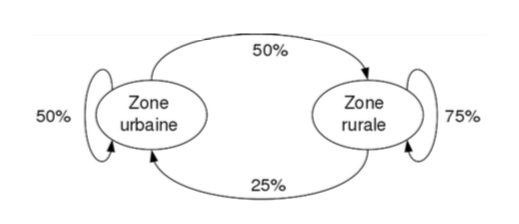
\includegraphics[scale=0.5]{migration.png}
    \end{center}
    Notos $r_0$ et $u_0$ la répartition initiale de la population en proportion. Notons $r_k$ la proportion de la population totale qui habite en zone rurale au terme de la $k$-ième année et $u_k$ la proportion de population qui habite en zone urbaine au terme de cette même année. S’agissant de proportion de population, on a, pour toute année $k$,
$$r_k + u_k = 1$$.
\begin{enumerate}
    \item  Écrire $r_{k+1}$ et $u_{k+1}$ en fonction $r_k$ et $u_k$
    \begin{solution}
        D'après le schéma de répartition, chaque année, on a
        $$
        u_{k+1}=\frac{1}{2}u_k + \frac{1}{4}r_k
        $$
        $$
        r_{k+1}=\frac{3}{4}r_k + \frac{1}{2}u_k
        $$.\\
        \hfill
\end{solution}
\item  Déterminer la matrice $A$ qui permet d'écrire la relation de la question précédente sous forme matricielle
    $$\begin{pmatrix} u_{k+1}\\r_{k+1}\end{pmatrix}=A.\begin{pmatrix} u_k\\r_k\end{pmatrix} $$
   \noindent $A$ est appelée la matrice de transition du système.
   
        \begin{solution}
       $$A=
       \begin{pmatrix}\frac{1}{2}&\frac{1}{4} \\ \frac{1}{2}& \frac{3}{4}\end{pmatrix}
        $$.
        \hfill
\end{solution}
   
    \item Montrer que 
     $$\begin{pmatrix} u_{k}\\r_{k}\end{pmatrix}=A^k.\begin{pmatrix} u_0\\r_0\end{pmatrix} $$

\begin{solution}
     $$\begin{pmatrix} u_{k}\\r_{k}\end{pmatrix}=A.\begin{pmatrix} u_{k-1}\\r_{k-1}\end{pmatrix}=A.A.\begin{pmatrix}u_{k-2}\\r_{k-2}\end{pmatrix}=...= A^k. \begin{pmatrix} u_0\\r_0\end{pmatrix} 
     $$.
     \hfill
\end{solution}

     \item Calculer les valeurs propres de $A$.
\begin{solution}
    Le polynôme caractéristique de $A$ est
    $$p(\lambda)=\mathrm{det}(A-\lambda.\mathrm{Id})=\mathrm{det}\begin{pmatrix}\frac{1}{2}-\lambda& \frac{1}{4}\\ \frac{1}{2}& \frac{3}{4}-\lambda\end{pmatrix}=(\frac{1}{2}-\lambda).(\frac{3}{4}-\lambda) - \frac{1}{8}=$$
    
    $$
    = \lambda^2 - \frac{5}{4}\lambda + \frac{1}{4}= (x-1)(x-\frac{1}{4})
    $$
    Donc $\lambda=1, \frac{1}{4}$.
\end{solution}


     \item Est-ce que $A$ est diagonalisable?
\begin{solution}
    Oui car d'après le théorème du cours, se $A$ admet des valeurs propres réels, $A$ est diagonalisable et il existe une matrice inversible P tel que
    $$
    A= P^{-1}.\begin{pmatrix}1& 0\\ 0& \frac{1}{4}\end{pmatrix}.P
    $$
\end{solution}

     \item Est-ce que la répartition de la population stabilise, c.à.d, est-ce que la limite
     
     $$
     \lim_{k\to\infty}\begin{pmatrix} u_{k}\\r_{k}\end{pmatrix}
     $$
     existe?
     
\begin{solution}
    D'après la question précèdent, 
    $$
    A^k= P^{-1}.\begin{pmatrix}1& 0\\ 0& \frac{1}{4}\end{pmatrix}^k.P= P^{-1}.\begin{pmatrix}1& 0\\ 0& \frac{1}{4^k}\end{pmatrix}.P= P^{-1}.\begin{pmatrix}1& 0\\ 0& 0\end{pmatrix}.P + \underbrace{\frac{1}{4^k}P^{-1}.\begin{pmatrix}0& 0\\ 0& 1\end{pmatrix}.P }_{\to 0 \text{ pour } k>>0 }
    $$
    
    $$
    \lim_{k\to \infty}A^k=P^{-1}.\begin{pmatrix}1& 0\\ 0& 0\end{pmatrix}.P
    $$
    
    Soit $U= P^{-1}.\begin{pmatrix}1& 0\\ 0& 0\end{pmatrix}.P$ et $V= P^{-1}.\begin{pmatrix}0& 0\\ 0& 1\end{pmatrix}.P$. \\
    
    On a un système
    $$
    \begin{cases}
    U+V= \mathrm{Id}\\
    U+ \frac{1}{4}V=A
    \end{cases}
    $$
    
    d'où:
    
    $$
    \frac{3}{4}U=A-\frac{1}{4}\mathrm{Id}
    $$
    
    $$
    U=\frac{1}{3}\begin{pmatrix} 1&1\\2&2\end{pmatrix}
    $$
    
    Donc, quand $k\to \infty$, on a 
    
    $$
    \lim_{k\to \infty} \begin{pmatrix} u_{k}\\r_{k}\end{pmatrix}= \lim_{k\to \infty} A^k. \begin{pmatrix} u_{0}\\r_{0}\end{pmatrix} = U.\begin{pmatrix} u_{0}\\r_{0}\end{pmatrix}=\frac{1}{3}\begin{pmatrix} 1&1\\2&2\end{pmatrix}.\begin{pmatrix} u_{0}\\r_{0}\end{pmatrix}=\frac{1}{3}\begin{pmatrix} u_{0}+r_{0}\\ 2u_0+2r_0\end{pmatrix}= \begin{pmatrix} \frac{1}{3}\\ \frac{2}{3}\end{pmatrix}
    $$
    A terme, il y aura donc un tiers de la population totale en zone urbaine et deux tiers en zone rurale. Notons que cette proportion est indépendante de la répartition initiale des populations entre les deux zones.
\end{solution}
\end{enumerate}
\end{exo}
 
 
 \begin{exo}
 [Espèces en compétition, \href{http://math.univ-lyon1.fr/homes-www/malbos/Ens/amalaa11.pdf}{Source}]
  On considère deux espèces A et B qui coexistent dans un même environnement naturel. On étudie deux situations d’évolution de ces espèces.
  
  \begin{itemize}
  \item Dans une première situation, on suppose que les deux espèces sont en compétition : le nombre d’individus d’une espèce augmente proportionnellement au nombre d’individus de cette même espèce et décroît proportionnellement au nombre d’individus de l’autre espèce.
 \begin{enumerate}
     \item Si la population de chaque espèce augmente de deux fois le nombre d’individus de l’espèce et décroît d’une fois le nombre d’individus de l’autre espèce, déterminer à chaque instant le nombre d’individus de chaque espèce lorsque initialement il y a 100 individus de l’espèce A et 200 individus de l’espèce B.
     
\begin{solution}
    On considère l'interaction entre les espèces $A$ et $B$ comme un système d'évolution en temps discret. Posons $A_0= 100$ et $B_0=200$ le nombre initial d'individus de chaque espèce et posons $A_k$ et $B_k$ le nombre d'individus de chaque espèce après k-étapes d'interaction.
    
    
    On a:
    
    $$\begin{cases}
    A_{k+1}=A_k + (2.A_k - B_k)= 3A_k - B_k\\
    B_{k+1}=B_k + (2.B_k- A_k)= 3B_k - A_k\\
    \end{cases}$$
    
    Donc, avec matrice de transition
    
    $$
    M=\begin{pmatrix}3&-1\\ -1& 3\end{pmatrix}
    $$
    
    Par récurrence, on obtient donc
    $$\begin{pmatrix} A_{k}\\B_{k}\end{pmatrix}=M^k.\begin{pmatrix} A_{0}\\B_{0}\end{pmatrix}=M^k.\begin{pmatrix} 100\\200\end{pmatrix}
     $$.
     
Les valeurs propres de $M$ sont $4$ et $2$. Donc, il existe une matrice inversible $P$ tel que

$$
M^k= P^{-1}\begin{pmatrix}4^k&0\\ 0& 2^k\end{pmatrix}.P
$$
    
\end{solution}     
     
     \item  Est-ce qu’une des espèces est en voie d'extinction? Si oui, au bout de combien de temps.
     
     
     
\begin{solution}

$$
\begin{pmatrix} A_{0}\\B_{0}\end{pmatrix}=
\begin{pmatrix} 100\\200\end{pmatrix},
\begin{pmatrix} A_{1}\\B_{1}\end{pmatrix}=
\begin{pmatrix} 100\\500\end{pmatrix},
\begin{pmatrix} A_{2}\\B_{2}\end{pmatrix}=
\begin{pmatrix} -200\\1400\end{pmatrix}
$$


Donc l'espèce $A$ est en voie d'extinction.
\end{solution}    


\end{enumerate}


 \item  Dans une deuxième situation, on suppose que les deux espèces vivent en symbiose de la façon suivante. Le nombre d’individus de chaque espèce augmente d’une fois le nombre d’individus de l’autre espèce et décroît d’une fois le nombre d’individus de la même espèce.
\begin{enumerate}
    \item Si initialement les espèces A et B sont respectivement composées de 200 et 400 individus, déterminer à chaque instant la population de chaque espèce.
    \item  Que se passe-t-il à long terme ?
\end{enumerate}
\end{itemize}
 \end{exo}
 
 \medskip
 
\begin{exo}[$\blacksquare$ Espèces en compétition, équilibre instable]
On considère une population de rats $R_k$ et de serpents $S_k$ à un instant $k$ donné où $k$ progresse par mois. On suppose que les populations évoluent selon les lois suivantes:

$$
S_{k+1}= 0.5S_k + 0.4R_k
$$

$$
R_{k+1}= -p S_k+ 1.1R_k
$$

\begin{itemize}
\item le facteur $0.5 S_k$ dans la première équation signifie que s'il n'y a pas de rats, seulement la moitié des serpents survivront le mois prochain. 
\item le facteur $1.1R_k$ signifie que s'il n'y a pas de serpents, la population des rats augmente de $10\%$ par mois. 
\item le terme $0.4R_k$
explique comment la population de rats aide la population de serpents à croître;
\item le paramètre $p>0$ c'est le taux de mortalité des rats, tués par les serpents
\end{itemize}

\begin{enumerate}
    \item Écrire la matrice $A$ qui décrit l'évolution du système en fonction de $p$.
\begin{solution}
    $$
    \begin{pmatrix}S_{k+1}\\ R_{k+1}\end{pmatrix}=\begin{pmatrix}
    0.5& 0.4\\-p&1.1
    \end{pmatrix}\begin{pmatrix}
    S_k\\ R_k
    \end{pmatrix}
    $$
\end{solution}
    \item Calculer les valeurs propres réels de $A$ en fonction de $p$.
\begin{solution}
    $$\mathrm{det}(\begin{pmatrix}
    0.5& 0.4\\-p&1.1
    \end{pmatrix}-\lambda.Id)=\mathrm{det}\begin{pmatrix}
    0.5-\lambda& 0.4\\-p&1.1-\lambda
    \end{pmatrix}= (0.5-\lambda).(1.1-\lambda)+0.4p= \lambda^2 - 1.6 \lambda + 0.55 + 0.4p$$
    
    $$\Delta=(-1.6)^2 - 4.(0.55+0.4p)=0.36 - 1.6p$$ 
    
    Donc pour avoir des valeurs propres réels il faut que 
    
    $$
    0.36-1.6p>0 \Leftrightarrow 1.6p<0.36 \Leftrightarrow p< 0.225
    $$
    Donc $\lambda_1= \frac{1.6+ \sqrt{0.36-1.6p}}{2}$ et $\lambda_2=\frac{1.6- \sqrt{0.36-1.6p}}{2}$.
\end{solution}
    \item Décrire l’évolution du système, ie, $\lim_{k\to+\infty} \begin{pmatrix}S_k\\R_k\end{pmatrix}$ lorsque:
\begin{enumerate}    
     \item $p=0.104$;
\begin{solution}
    Pour $p=0.104$, on trouve $\lambda_1= 1.02$ et $\lambda_2=0.58$. Vue que $\lambda_1>1>\lambda_2>0$,
    la valeur propre $\lambda_2=0.58$ n'a pas de contribution asymptotique. Comme $\lambda_1>1$, le deux populations vont proliférer.
\end{solution}
    \item $p=0.2$;
\begin{solution}
    Pour $p=0.2$, on trouve $\lambda_1= 0.9$ et $\lambda_2=0.7$. Comme les deux valeurs propres sont positives et inférieurs à 1, 
les deux espèces vont disparaître. Voir 
\href{https://www.wolframalpha.com/input/?i=u%28n%2B1%29%3D0.5*u%28n%29%2B0.4*v%28n%29%2C+v%28n%2B1%29%3D-0.2*u%28n%29%2B%281.1%29*v%28n%29}{Lien Wolframalpha}. 
Voici les résultats pour $S_0=10$ et $R_0=100$:

\begin{figure}[H]
\begin{center}
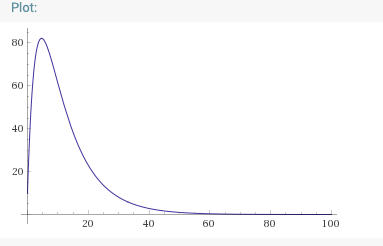
\includegraphics[scale=0.5]{serpentsp02.png}
\caption{Serpents}
\end{center}
\end{figure}
        
        \begin{figure}[H]
        \begin{center}
         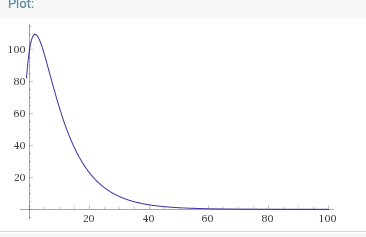
\includegraphics[scale=0.5]{ratsp02.png}
        \caption{Rats}
        \end{center}
        \end{figure}




\end{solution}
    \item $p=0.125$;
\begin{solution}
    Pour $p=0.125$, on trouve $\lambda_1= 1.0$ (avec vecteur propre $(\frac{4}{5},1)$) et $\lambda_2=0.6$ (avec vecteur propre $(4,1)$).Comme $0<\lambda_2<1$, il y a que la contribution de $\lambda_1$. Mais $\lambda_1=1$ implique que les deux populations seront en équilibre, c'est à dire, les effectifs de chaque population resteront constants. Voici les résultats pour une population iniciale de $S_0=10, R_0=100$:
    

\begin{figure}[H]
\begin{center}
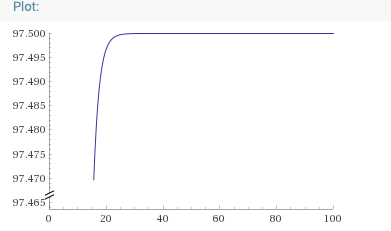
\includegraphics[scale=0.5]{serpentsp0125.png}
\caption{Serpents}
\end{center}
\end{figure}
        
        \begin{figure}[H]
        \begin{center}
         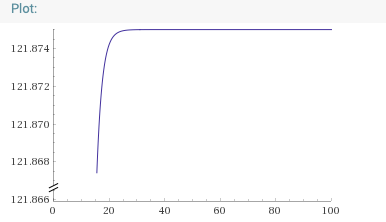
\includegraphics[scale=0.5]{ratsp0125.png}
        \caption{Rats}
        \end{center}
        \end{figure}
    
    
    Cependant, c'est un équilibre instable, dans le sens où une petite variation du paramètre $p$ (par exemple, par une nouvelle maladie des serpents), peut nous faire revenir soit à l'extinction (4), soit à la prolifération (1). 
\end{solution}
\end{enumerate}
\end{enumerate}
\end{exo}
 
 
\section{Limites Énergétiques}

\begin{exo}[Pic pétrolier]
La quantité de pétrole disponible sur la planète est gigantesque mais finie, disons, $Q$. Avant 1700, nous n'avons pas utilisé de pétrole. Soit  donc  $C(t)$ la quantité de pétrole consommé  par l'humanité pendant l'année $1700+t$. On suppose que  $C(0)=0$ et que $C(t)$ est continue.
\begin{enumerate}
    \item On suppose que la limite $\lim_{t\to +\infty} C(t)$ existe. En utilisant le fait que la quantité disponible de pétrole est finie, montrer que cette limite vaut 0.
   
   
  \begin{solution}
  La quantité totale de pétrole utilisé entre 1700 et 1700+T est donnée par l'intégrale
    $$
    \int_{0}^T C(t).dt
    $$
    et par hypothèse, 
    $$
    \lim_{T\to +\infty}\int_{0}^T C(t)dt=Q
    $$
    On raisonne par l'absurde:
 supposons que la limite $\lim_{t\to +\infty} C(t)$ existe et  vaut $L \neq 0$. Comme $C$ est positive, alors $L\geq 0$. Donc on a $L>0$, alors il existe $N\in [0, +\infty[$ tel que pour $t>N$, $C(t)>\frac L2$.On en déduit que $\int_{N}^{t}C(t)dt> (t-N)*\frac L2$. C'est en contradiction avec  $$
    \lim_{T\to +\infty}\int_{0}^T C(t).dt=Q
    $$
\end{solution}
    
    
 \item Montrer que sous la condition $\lim_{t\to +\infty} C(t)=0$ la fonction $C(t)$ admet un maximum absolue.
 
\begin{solution}
  Ici on utilise le théorème des bornes atteintes. En effet, la fonction $C(t)$ est continue est non-nulle, donc il existe $a\in [0, +\infty[$ tel que $C(a)\neq 0$. Par la question 1), $\lim_{t\to +\infty} C(t)=0$, et donc, il existe $N\geq 0$ tel que $\forall t> a, C(t)< C(a)$. Prenons donc l'intervalle fermée $[0, N]$. Ici, par le théorème des bornes atteintes, $C(t)$ admet un maximum absolue. Donc, $C(t)$ admet un maximum absolue sur $[0, +\infty[$.
\end{solution}
 
  \end{enumerate}  
\end{exo}
  
\medskip


\begin{exo}[Épuisement des ressources et croissance]
En 1900, la quantité totale d'énergie consommée par l'humanité était d'environ $5 \times 10^3$ Twh. Depuis 1900, le taux de croissance de la consommation d’énergie est en moyenne d’environ 3$\%$ par an. 
\begin{enumerate}
\item Si on fixe 1900 comme l'année zéro, donner la formule pour $E(t)$ la quantité d'énergie consommée par l'humanité pendant l'année 1900+t.

\begin{solution}
$E(t)=E_0(1+0,03)^t= E_0\, e^{\log (1,03)t}= 5 10^3 e^{\log (1,03)t}$.
\end{solution}
   
\item Calculer la quantité d'énergie consommée par l'humanité en 2013 (vous pouvez comparer avec les informations qu'on trouve sur  Internet).

\begin{solution}
    La formule de la question précédente donne $E(113) \simeq 10^5$ Twh.
\end{solution}

   \item L'intégralité de l'énergie consommée entre 1900 et 1900+T est donnée par l'intégrale
     $$Q(T)= \int_{0}^T E(t).dt$$
     Le calculer explicitement.
     
\begin{solution}
     $$Q(T)= \int_{0}^T E(t).dt= \int_{0}^t E_0\, e^{\log (1,03)t}.dt=E_0 \int_{0}^T \, e^{\log (1,03)t}.dt $$
     $$
     = \log (1,03).E_0 [ e^{\log (1,03)t}]_{0}^{T}= \log (1,03).E_0.(e^{\log (1,03)T}-1)
     $$
\end{solution}

    \item  Il est facile d'imaginer (bitcoin, netflix, 5G, etc), la consommation d'énergie pendant le 21ème siècle pourrait continuer de croître de la même manière. La terre a des ressources finies - la quantité totale d'énergie stockée est peut être estimée par l'équation d'Einstein $E_T = m_T.c^2$, où $m_T$ est la masse terrestre (environ $6\times 10^{24} kg$) et $c$ est la vitesse de la lumière $3 10^8$ m/s. Combien de siècles nous avons avant de consommer la totalité de l'énergie terrestre? Comparer avec l'âge de la Terre.
    
\begin{solution}
    Il faut d'abord calculer $E_T=m_T. c^2= 5\times 10^{35}$ J $\sim 10^{26}$ Twh. Il faut maintenant résoudre l'équation
     $$
     \log (1,03)*(5000).((1,03)^T-1)=10^{26}
     $$
     
     On trouve 
     $$T=1856\sim 18,5 \,\text{siècles}$$
     
\end{solution}
\end{enumerate}
\end{exo}







\begin{exo}[EROI - Taux de retour énergétique et le prix du pétrole, \href{https://www.sciencedirect.com/science/article/pii/S0301421511006975}{Source ici}]
Pour produire du pétrole on a besoin d'énergie pour faire  fonctionner les machines d'extraction. Plus précisément, si $E_T$ c'est la quantité totale d'énergie extraite en équivalent pétrole, il y a une partie $E_{M}$ d'énergie qu'il faut redonner aux machines d'extraction et une partie $E_{L}$ qu'on peut livrer dans l'économie.

\begin{center}
\begin{tikzpicture}
    \node at (0,0) (Extraction du pétrole) {Extraction du pétrole};
    \node at (7,0) (here) {$E_L$};
    \node at (3,2.5) (lalonge) {$E_M$};
     \node at (5,0) (there) {$E_T$};
    \draw [->, line width=3mm] (Extraction du pétrole) to[out=0, in=180,looseness=2] (there);
     \draw [->, red, line width=1mm] (there) to[out=60, in=90,looseness=2] (Extraction du pétrole)  ; 
     \draw [->, blue, line width=2mm] (there) to[out=0, in=180,looseness=2] (here); 
\end{tikzpicture}
\end{center}


$$E_T= E_{M}+ E_{M}$$


Nous définissons le taux de retour énergétique EROI comme le ratio
$$
EROI=\frac{E_{T}}{E_{M}}
$$

\begin{itemize}
    \item Si $P$ est le prix moyen par unité d’énergie, on a un bénéfice total donnée par
    $$ P. E_{L}$$
    
    \item Si $C$ c'est le coût moyen de production par unité d'énergie, le coût total de production est donnée par 
    $$
    C. E_{T}
    $$
    \item La marge de bénefice $m$ est donnée par
    $$
    m=\frac{P. E_{L}}{C. E_{T}}
    $$
    

    
\end{itemize}

\begin{enumerate}
    \item Montrer que
    $$
    P=\frac{m.C}{(1-\frac{1}{EROI})}
    $$

\begin{solution}
    On a $$P. E_{L}= m.C.E_T=m.C.\frac{E_T}{E_L}=m.C.\frac{E_T}{E_T-E_M}=m.C.\frac{1}{(1-
    \frac{E_M}{E_T})}=\frac{m.C}{(1-
    \frac{1}{EROI})}$$
\end{solution}
    
   
    \item Supposons maintenant que  le produit $m.C$ reste constant. 
    
   
    
    \begin{enumerate}
        \item Calculer
    $$
    \lim_{EROI\to 0} P\,\,\,, \,\, \lim_{EROI\to 1^-} P\,\,\,, \,\,\,  \lim_{EROI\to 1^{+}} P\,\,\,, \,\,\,  \lim_{EROI\to +\infty} P
    $$
\begin{solution}
$$\lim_{EROI\to 0} P=\frac{m.C}{(1-
    \underbrace{\frac{1}{EROI}}_{\to +\infty})}\to 0^-$$

$$\lim_{EROI\to 1^-} P=\frac{m.C}{\underbrace{(1-
    \underbrace{\frac{1}{EROI}}_{\to 1^+})}_{\to 0^-}}\to -\infty $$
    
$$\lim_{EROI\to 1^-} P=\frac{m.C}{\underbrace{(1-
    \underbrace{\frac{1}{EROI}}_{\to 1^-})}_{\to 0^+}}\to +\infty $$
    
$$\lim_{EROI\to +\infty} P=\frac{m.C}{\underbrace{(1-
    \underbrace{\frac{1}{EROI}}_{\to 0})}_{\to 1}}\to m.C $$
    

        
\end{solution}
    
    \item Calculer la dérivée $P'$ pour $EROI\in ]1,+\infty[$ et le tableau de variation de $P$ en fonction de l'EROI.
    
    
\begin{solution}
$$P'=\frac{-mC}{(EROI-1)^2}\,\,\,\,\,\, \text{ donc } P'<0$$

\end{solution}


    \item Dessiner le graphe de $P$ en fonction de l'EROI entre $]1,+\infty]$.
    
\begin{solution}
	\begin{center}
	\begin{tikzpicture}[scale = .5]
		\draw[->] (-0.5,0) -- (7,0) node[below] {$EROI$};
		\draw[->] (0,-.5) -- (0,4) node[right=-0.05cm] {$P$};
		\draw[domain=1.4:6,samples=200,color=blue] plot ({\x},{1/(1-1/\x)}); 
		\end{tikzpicture}
	\end{center}
\end{solution}    
    

\item Conclure que même si le coût de production $C$ et la marge de bénéfice $m$ restant constants, c'est possible, à cause de la diminution de  l'EROI, que le prix de vente explose très vite.

\item En 1965, L'EROI était de 19.5 et depuis on observe que en fonction du temps (par an), on a

$$EROI(t)= 19.5 - 0.25.t$$

Étudier le prix $P$ en fonction de $t$.

    \end{enumerate}
\end{enumerate}




\end{exo}

\section{Hypothèses mathématiques irréalistes en économie}


\begin{exo}[$\blacksquare$ Le paradoxe de Jevons (Effet rebond)]
Le paradoxe de Jevons énonce qu'à mesure que les améliorations technologiques augmentent l'efficacité avec laquelle une ressource est employée, la consommation totale de cette ressource peut augmenter au lieu de diminuer.
\end{exo}

\begin{exo}[$\blacksquare$ Le prix nobel de Nordhaus pour la relation PIB/temperature, voir le \href{https://www.youtube.com/watch?v=vwwvZ8g5eHE}{Lien}]Le prix Nobel d'économie de 2018 a été décerné aux Américains William Nordhaus et Paul Romer, pour leurs travaux sur l'intégration du changement climatique et de l'innovation technologique dans l'analyse macro-économique. Voici leurs prévisions pour l'impact provoqué par l'augmentation de température sur le PIB mondial:

\begin{center}
    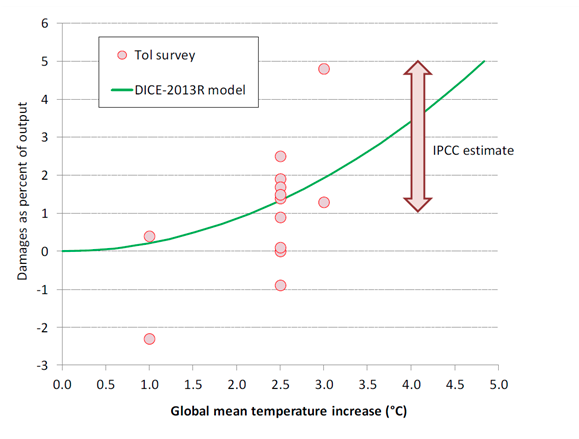
\includegraphics[scale=0.5]{nordhaus.png}
\end{center}


Pour faire ce calcul, ils supposent que l'impact ("damage") $D(T)$ provoqué par une augmentation de température de $T$ dégrées est quadratique

$$
D(T)=0.00267 T^2
$$

\begin{enumerate}
    \item Montrer que $D(T)$ est continue.
\begin{solution}
    $D(T)$ est polynomiale donc continue.
\end{solution}


\item D'après le graphe ci-dessus on constate que pour une différence de température de $T=4$ dégrées, l'impact sur le PIB mondial est de $3,5\%$. Comparer avec l'impact de la crise de 2008 sur le PIB mondial.

\begin{solution}
    D'après les économistes, la crise de 2008 a eu un impact d'environ $4\%$ sur le PIB mondial.
\end{solution}


\item La différence entre les deux images correspond à une augmentation de la température mondiale d'environ $T=4$ degrés:

\begin{center}
    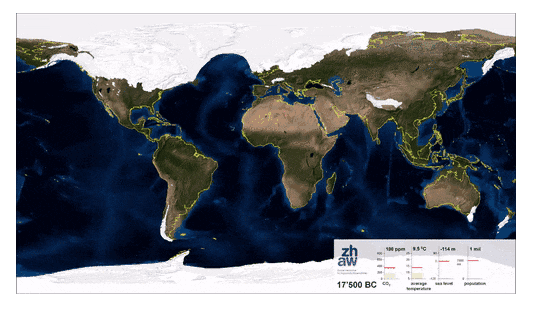
\includegraphics[scale=0.5]{before}
\end{center}

\begin{center}
    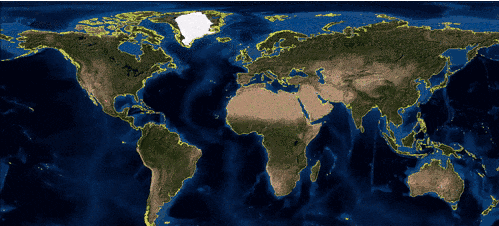
\includegraphics[scale=0.5]{now}
\end{center}


Est-il raisonnable de penser que cela aura moins d'impact que la crise de 2008?
\medskip


\item Un point de basculement dans le système climatique est un seuil qui, lorsqu'il est dépassé, peut entraîner de grands changements dans l'état du système.  Voici une version modifié de la fonction d'impact de Nordhaus avec un point de basculement en $T=4$ dégrées:

$$
D_b(T)= \frac{0.008 T^3}{4-T}
$$

\begin{enumerate}
    \item Montrer que $D_b(1)=D(1)$ et que jusqu'à 1 dégrée de plus, les deux modèles sont comparables.
    \item Calculer $\lim_{T\to 4} D_b(T)$. Est-ce que $D_b(T)$ est continue en $T=4$?
    \item Comparer les graphes de $D_b$ et $D$ et discuter la  plausibilité physique des deux.
\end{enumerate}

\begin{solution}

    \begin{center}
        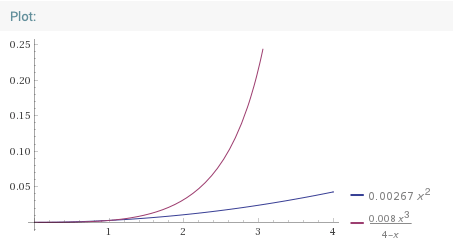
\includegraphics[scale=0.8]{nordhausfunctioncorrected.png}
    \end{center}
\end{solution}


\end{enumerate}





\end{exo}












\begin{exo}[Multiplicité d'équilibres]
L'économie d'un certain pays est composée de trois secteurs: énergie E, métallurgie $M$ et charbon $C$.  Chaque secteur doit utiliser une partie de sa propre production et vendre la partie qui reste aux autres secteurs.
Le schéma suivant résume ces informations en $\%$ de production.


\begin{figure}[H]
\centering
\begin{tikzpicture}[->,auto,node distance=4cm,
  thick,main node/.style={circle,draw,font=\sffamily\Large\bfseries}]

\node[main node] (E) {Énergie};
\node[main node] (M) [below left of=E] {Métallurgie};
\node[main node] (C) [below right of=E] {Charbon};

\draw [->]  (E) to [out=30,in=150, looseness=4]   node[above] {0.1} (E) ;
\draw [->] (M) to [out=-150,in=150, looseness=4]  node[left] {0.2} (M);
\draw [->] (C) to [out=-30,in=30, looseness=4]  node[right] {0} (C);

\path[every node/.style={font=\sffamily\small}]
    (E) edge [right] node[above]  {0.5} (M)
    (E) edge node[midway] [right] {0.4} (C)
(M) edge [bend right] node[midway] [right] {0.2} (E)
    (M) edge [right] node[above]  {0.6} (C)
        (C) edge[bend right] node[midway] [right] {0.6} (E)
        
    (C) edge[bend left]  node[below]  {0.4} (M);
\end{tikzpicture}
\end{figure}


On note que pour chaque secteur, la somme des portions sortants est égale à 1. Notons $p_E$, $p_M$ et $p_C$ le chiffre d'affaires de chaque secteur.
 
 
 \begin{enumerate}
 \item Traduire en termes d'un système d'équations linéaire la condition d'équilibre budgétaire simultanée pour les trois secteurs.
 \begin{solution}
 Pour que le secteur du charbon soit en équilibre budgétaire , il faut que 
 $$p_C= 0.6 p_M+ 0.4.p_E$$
 Pour le secteur de l'énergie on a besoin de 
 $$
 p_E=0.1p_E+ 0.2p_M+ 0.6p_C
 $$
 Finalement, pour le secteur métallurgique
 $$
 p_M=0.5p_E+ 0.2p_M+ 0.4p_C
 $$
 On obtient donc le système linéaire:
 $$
 \begin{cases}
  p_C- 0.4p_E - 0.6p_M=0\\
- 0.6p_C +0.9p_E- 0.2p_M =0\\
-0.4p_C - 0.5p_E+0.8p_M =0
 \end{cases}
 $$

 

 
\end{solution}
 \item Est-ce qu'une tel condition d'équilibre existe et est unique?
\begin{solution}
La matrice augmentée:  $$
\begin{amatrix}{3} 1&-0.4& -0.6 & 0 \\ -0.6&0.9 & -0.2 & 0 \\ -0.4&-0.5 & 0.8  & 0 \end{amatrix}
$$
Par pivot de Gauss, on obtient

 $$
\begin{amatrix}{3} 1&-0.4& -0.6 & 0 \\ 0&0.66 & -0.56 & 0 \\ 0&-0.66 & 0.56  & 0 \end{amatrix}\to \begin{amatrix}{3} 1&-0.4& -0.6 & 0 \\ 0&0.66 & -0.56 & 0 \\ 0&0& 0 & 0 \end{amatrix}\to \begin{amatrix}{3} 1&-0.4& -0.6 & 0 \\ 0&1 & -0.85 & 0 \\ 0&0& 0 & 0 \end{amatrix}\to\begin{amatrix}{3} 1&0& -0.94 & 0 \\ 0&1 & -0.85 & 0 \\ 0&0& 0 & 0 \end{amatrix}
$$

Donc,

 $$
 \begin{cases}
  p_C= 0.94 p_M\\
p_E=0.85 p_M\\
p_M\text{ variable libre}
 \end{cases}
 $$


Conclusion: il y a une infinité de points d'équilibre, un pour chaque choix de $p_M$


\end{solution}
 \end{enumerate}
\end{exo}


\end{document}
